%*******************************************************************************
%****************************** Second Chapter *********************************
%*******************************************************************************

\chapter{Tecnologie utilizzate}
\label{cap:2}
Il presente capitolo descrive le principali tecnologie e i concetti teorici che costituiscono la base del lavoro di analisi e confronto sviluppato nei capitoli successivi. L’obiettivo è fornire un inquadramento completo degli strumenti e delle metodologie adottate, con particolare attenzione ai paradigmi di \textbf{apprendimento automatico}, ai \textbf{modelli linguistici di grandi dimensioni} e alle \textbf{tecniche di ottimizzazione dell’apprendimento} oggetto della tesi.


\section{Large Language Models}
I \textbf{Large Language Models} (LLM) rappresentano l'attuale stato dell'arte nell'elaborazione del linguaggio naturale (NLP). Essi si basano su architetture di Deep Learning, specificamente il \textbf{Transformer} introdotto da \citet{vaswani2017attention}, che ha rivoluzionato il campo grazie all'introduzione del meccanismo di \textit{self-attention}. Tale meccanismo permette al modello di elaborare le sequenze di dati in parallelo e di catturare dipendenze a lungo raggio all'interno del testo, superando i limiti intrinseci delle precedenti architetture ricorrenti (RNN).

La caratteristica distintiva dei Large Language Models risiede nella scala: essi sono composti da miliardi di parametri e vengono addestrati su \textbf{dataset} di dimensioni colossali (nell'ordine dei Terabyte). Questa crescita esponenziale della complessità ha dato origine alle cosiddette \textbf{capacità emergenti}: abilità, come il ragionamento logico e la risoluzione di problemi complessi, che si manifestano una volta superata una certa soglia di dati e parametri.

Tuttavia, i modelli matematici non sono in grado di elaborare direttamente il testo grezzo. Per questo motivo, i dati vengono sottoposti a un processo di \textbf{tokenizzazione}. La tokenizzazione consiste nella scomposizione del testo in unità minime chiamate \textit{token}, che possono corrispondere a intere parole, sottoparole o singoli caratteri. Attraverso algoritmi come il \textit{Byte Pair Encoding} (BPE), ogni token viene mappato in un indice numerico all'interno di un vocabolario predefinito. Questi indici vengono poi convertiti in vettori densi di numeri reali, detti \textbf{embeddings}, che permettono al modello di operare in uno spazio semantico dove parole con significati simili si trovano matematicamente vicine.

\begin{comment} PER RICORDARE COM'ERA LA FORMATTAZIONE PRIMA DELLA MODIFICA DELLE IMMAGINI
\subsection{L'architettura Transformer}
\label{subsec:transformer}

L'introduzione dell'architettura \textbf{Transformer}, formalizzata da \citet{vaswani2017attention} attraverso il fondamentale articolo \textit{"Attention is All You Need"}, ha rappresentato un cambiamento di paradigma senza precedenti nel campo dell'elaborazione del linguaggio naturale (NLP). Prima della sua diffusione, lo stato dell'arte era dominato dalle reti neurali ricorrenti (RNN) e dalle loro varianti, come le \textit{Long Short-Term Memory} (LSTM) \cite{hochreiter1997long}, le quali elaboravano le sequenze di dati in modo intrinsecamente sequenziale. Tale approccio presentava due limitazioni critiche: la difficoltà nel gestire dipendenze a lungo raggio a causa del fenomeno della scomparsa del gradiente e l'impossibilità di parallelizzare efficacemente il calcolo, rendendo l'addestramento su grandi dataset estremamente oneroso in termini temporali. Il Transformer risolve radicalmente queste problematiche abbandonando la ricorsività a favore di un'architettura basata esclusivamente sul meccanismo di attenzione.

Il pilastro teorico e funzionale di questa architettura è rappresentato dal meccanismo di \textbf{Self-Attention} (auto-attenzione), un processo che permette al modello di esaminare ogni parola all'interno di una sequenza e determinare, attraverso un sistema di pesi dinamici, quali altri token siano più rilevanti per comprenderne il contesto, indipendentemente dalla loro distanza fisica nel testo. Da un punto di vista matematico, questa operazione si realizza proiettando ogni token di input in tre diversi spazi vettoriali, generando così tre matrici: la \textbf{Query} ($Q$), che rappresenta il token attuale in cerca di contesto; la \textbf{Key} ($K$), che contiene le informazioni salienti di tutti i token della sequenza; e il \textbf{Value} ($V$), che racchiude il contenuto informativo effettivo. L'interazione tra questi elementi avviene attraverso il calcolo del prodotto scalare tra Query e Key, il cui risultato viene normalizzato per determinare quanto peso assegnare a ciascun valore. La funzione di attenzione è definita formalmente come:

\begin{equation}
	\text{Attention}(Q, K, V) = \text{softmax}\left(\frac{QK^T}{\sqrt{d_k}}\right)V
\end{equation}

In questa espressione, il termine $\sqrt{d_k}$, dove $d_k$ è la dimensione delle chiavi, funge da fattore di scala cruciale per evitare che il prodotto scalare assuma valori eccessivamente elevati, i quali porterebbero la funzione softmax in regioni con gradienti estremamente piccoli, ostacolando l'apprendimento.



Per aumentare la capacità espressiva del modello, il Transformer non si limita a un singolo calcolo di attenzione, ma impiega la cosiddetta \textbf{Multi-Head Attention}. Questa tecnica consiste nell'eseguire molteplici operazioni di attenzione in parallelo, ognuna con i propri parametri lineari appresi; ciò consente al sistema di "osservare" la sequenza da diverse prospettive semantiche e sintattiche simultaneamente, catturando relazioni complesse che un unico meccanismo di attenzione non riuscirebbe a isolare. Tuttavia, la natura parallela del Transformer comporta la perdita intrinseca dell'informazione sull'ordine temporale delle parole, un elemento invece naturale nelle RNN. Per sopperire a questa mancanza, vengono introdotti i \textbf{Positional Encoding}, segnali sinusoidali di diversa frequenza che vengono sommati ai vettori di embedding iniziali. Tali segnali forniscono al modello una coordinata spaziale per ogni token, permettendogli di distinguere tra frasi con le stesse parole disposte in ordini differenti.


\begin{figure}[htbp]
	\centering
	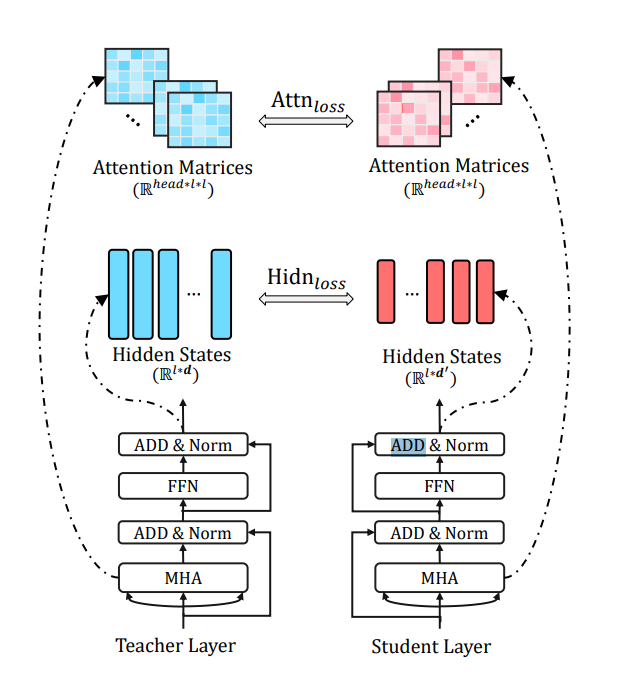
\includegraphics[width=0.5\textwidth]{Figs/MHA.png} 
	\caption{\small Dettagli del processo di distillazione a livello di strato del Transformer. La procedura integra la distillazione basata sull'attenzione ($Attn_{loss}$), calcolata sulle matrici di attenzione, e la distillazione basata sugli stati nascosti ($Hidn_{loss}$), applicata alle rappresentazioni latenti tra lo strato insegnante (\textit{Teacher Layer}) e lo strato studente (\textit{Student Layer}).}
	\label{fig:distillazione_transformer}
\end{figure}


Oltre ai moduli di attenzione, ogni blocco dell'architettura integra reti neurali di tipo \textit{feed-forward} che operano in modo indipendente su ciascuna posizione, garantendo una trasformazione non lineare delle rappresentazioni apprese. La stabilità dell'addestramento e la possibilità di stratificare decine di questi blocchi (dando vita a modelli estremamente profondi) sono assicurate dall'integrazione di connessioni residue (\textit{residual connections}) seguite da fasi di \textit{Layer Normalization}. Queste strutture permettono ai gradienti di fluire più agevolmente durante la retropropagazione, mitigando i rischi di degradazione del modello. In ultima analisi, la straordinaria efficacia del Transformer risiede proprio nella sua scalabilità e nell'efficienza computazionale derivante dalla parallelizzazione massiva, proprietà che hanno permesso di addestrare i moderni \textit{Large Language Models} su corpora di dimensioni globali, rendendo necessario, in fase di implementazione pratica, il ricorso a tecniche di ottimizzazione come la \textit{Knowledge Distillation} per bilanciare l'enorme complessità parametrica con le risorse hardware disponibili.
\end{comment}

\subsection{L'architettura Transformer}
\label{subsec:transformer}

L'introduzione dell'architettura \textbf{Transformer}, formalizzata da \citet{vaswani2017attention} attraverso il fondamentale articolo \textit{"Attention is All You Need"}, ha rappresentato un cambiamento di paradigma senza precedenti nel campo dell'elaborazione del linguaggio naturale (NLP). Prima della sua diffusione, lo stato dell'arte era dominato dalle reti neurali ricorrenti (RNN) e dalle loro varianti, come le \textit{Long Short-Term Memory} (LSTM) \cite{hochreiter1997long}, le quali elaboravano le sequenze di dati in modo intrinsecamente sequenziale. Tale approccio presentava due limitazioni critiche: la difficoltà nel gestire dipendenze a lungo raggio a causa del fenomeno della scomparsa del gradiente e l'impossibilità di parallelizzare efficacemente il calcolo, rendendo l'addestramento su grandi dataset estremamente oneroso in termini temporali. Il Transformer risolve radicalmente queste problematiche abbandonando la ricorsività a favore di un'architettura basata esclusivamente sul meccanismo di attenzione.

Il pilastro teorico e funzionale di questa architettura è rappresentato dal meccanismo di \textbf{Self-Attention} (auto-attenzione), un processo che permette al modello di esaminare ogni parola all'interno di una sequenza e determinare, attraverso un sistema di pesi dinamici, quali altri token siano più rilevanti per comprenderne il contesto, indipendentemente dalla loro distanza fisica nel testo. Da un punto di vista matematico, questa operazione si realizza proiettando ogni token di input in tre diversi spazi vettoriali, generando così tre matrici: la \textbf{Query} ($Q$), che rappresenta il token attuale in cerca di contesto; la \textbf{Key} ($K$), che contiene le informazioni salienti di tutti i token della sequenza; e il \textbf{Value} ($V$), che racchiude il contenuto informativo effettivo. L'interazione tra questi elementi avviene attraverso il calcolo del prodotto scalare tra Query e Key, il cui risultato viene normalizzato per determinare quanto peso assegnare a ciascun valore. La funzione di attenzione è definita formalmente come:

\begin{equation}
	\text{Attention}(Q, K, V) = \text{softmax}\left(\frac{QK^T}{\sqrt{d_k}}\right)V
\end{equation}

In questa espressione, il termine $\sqrt{d_k}$, dove $d_k$ è la dimensione delle chiavi, funge da fattore di scala cruciale per evitare che il prodotto scalare assuma valori eccessivamente elevati, i quali porterebbero la funzione softmax in regioni con gradienti estremamente piccoli, ostacolando l'apprendimento.



Per aumentare la capacità espressiva del modello, il Transformer non si limita a un singolo calcolo di attenzione, ma impiega la cosiddetta \textbf{Multi-Head Attention}. Questa tecnica consiste nell'eseguire molteplici operazioni di attenzione in parallelo, ognuna con i propri parametri lineari appresi; ciò consente al sistema di "osservare" la sequenza da diverse prospettive semantiche e sintattiche simultaneamente, catturando relazioni complesse che un unico meccanismo di attenzione non riuscirebbe a isolare. Tuttavia, la natura parallela del Transformer comporta la perdita intrinseca dell'informazione sull'ordine temporale delle parole, un elemento invece naturale nelle RNN. Per sopperire a questa mancanza, vengono introdotti i \textbf{Positional Encoding}, segnali sinusoidali di diversa frequenza che vengono sommati ai vettori di embedding iniziali. Tali segnali forniscono al modello una coordinata spaziale per ogni token, permettendogli di distinguere tra frasi con le stesse parole disposte in ordini differenti.


\begin{figure}[t]
	\centering
	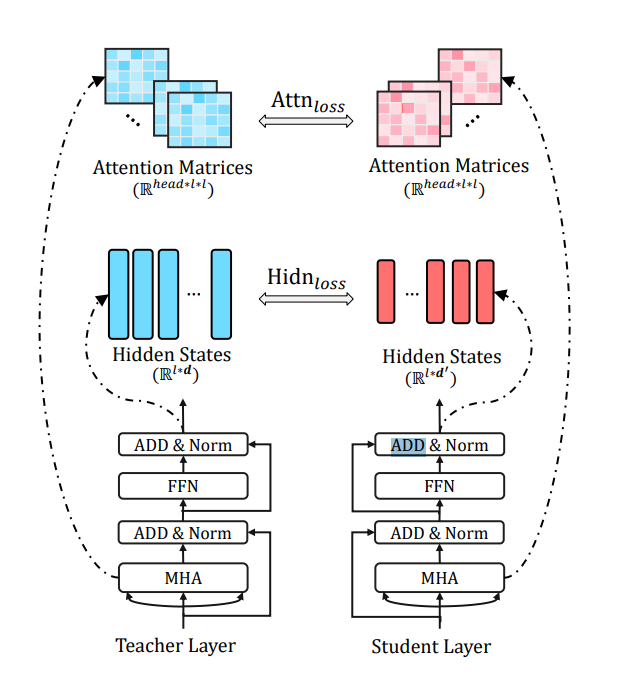
\includegraphics[width=0.5\textwidth]{Figs/MHA.png} 
	\caption{\small Dettagli del processo di distillazione a livello di strato del Transformer. La procedura integra la distillazione basata sull'attenzione ($Attn_{loss}$), calcolata sulle matrici di attenzione, e la distillazione basata sugli stati nascosti ($Hidn_{loss}$), applicata alle rappresentazioni latenti tra lo strato insegnante (\textit{Teacher Layer}) e lo strato studente (\textit{Student Layer}).}
	\label{fig:distillazione_transformer}
\end{figure}


Oltre ai moduli di attenzione, ogni blocco dell'architettura integra reti neurali di tipo \textit{feed-forward} che operano in modo indipendente su ciascuna posizione, garantendo una trasformazione non lineare delle rappresentazioni apprese. La stabilità dell'addestramento e la possibilità di stratificare decine di questi blocchi (dando vita a modelli estremamente profondi) sono assicurate dall'integrazione di connessioni residue (\textit{residual connections}) seguite da fasi di \textit{Layer Normalization}. Queste strutture permettono ai gradienti di fluire più agevolmente durante la retropropagazione, mitigando i rischi di degradazione del modello. In ultima analisi, la straordinaria efficacia del Transformer risiede proprio nella sua scalabilità e nell'efficienza computazionale derivante dalla parallelizzazione massiva, proprietà che hanno permesso di addestrare i moderni \textit{Large Language Models} su corpora di dimensioni globali, rendendo necessario, in fase di implementazione pratica, il ricorso a tecniche di ottimizzazione come la \textit{Knowledge Distillation} per bilanciare l'enorme complessità parametrica con le risorse hardware disponibili.

\subsection{Pre-training}

Il \textbf{Pre-training} costituisce la fase iniziale e computazionalmente più onerosa del ciclo di vita di un Large Language Model (LLM). In questa fase, il modello viene addestrato su una vastissima mole di dati non etichettati (\textit{unlabelled data}) provenienti da fonti eterogenee quali il web (ad esempio Common Crawl), libri, articoli scientifici, documentazione tecnica e codice sorgente. Con il termine \textbf{unlabelled data} si fa riferimento a informazioni grezze prive di una \textit{ground truth} definita a priori; il modello, pertanto, non riceve istruzioni esplicite sul significato dei dati da parte di un supervisore umano, ma è chiamato a inferirne autonomamente le regolarità statistiche e le strutture latenti.
L'obiettivo primario del pre-training è l'apprendimento \textbf{self-supervised learning} (\textit{self-supervised learning}), generalmente implementato attraverso il task di \textit{Next Token Prediction}. In questo contesto, dato un contesto testuale parziale, il modello deve stimare la distribuzione di probabilità del token successivo, aggiornando i propri parametri in modo da minimizzare una funzione di perdita, tipicamente la \textit{cross-entropy loss}. Sebbene il compito appaia semplice, la sua ripetizione su miliardi o trilioni di esempi consente al modello di apprendere relazioni sintattiche, strutture grammaticali complesse, dipendenze semantiche a lungo raggio e, in maniera implicita, una vasta conoscenza enciclopedica del mondo.
Un aspetto cruciale del pre-training riguarda la \textbf{preparazione e la curazione dei dati}. Prima dell’addestramento, i dataset vengono sottoposti a processi di filtraggio, deduplicazione e normalizzazione al fine di ridurre il rumore, eliminare contenuti ridondanti e migliorare la qualità complessiva delle informazioni. Successivamente, il testo viene trasformato in una sequenza di token tramite tecniche di \textbf{tokenizzazione} (come Byte Pair Encoding o Unigram Language Model), che consentono di rappresentare il linguaggio naturale in una forma numerica trattabile dalle reti neurali.
Dal punto di vista computazionale, il pre-training richiede infrastrutture hardware altamente specializzate, basate su GPU o TPU, e strategie di ottimizzazione avanzate come il \textit{data parallelism} e il \textit{model parallelism}. La letteratura ha inoltre evidenziato l’esistenza di \textbf{scaling laws}, secondo cui le prestazioni del modello migliorano in modo prevedibile all’aumentare della quantità di dati, del numero di parametri e delle risorse computazionali impiegate. Tuttavia, tali benefici sono accompagnati da costi energetici ed economici significativi, rendendo il pre-training una fase accessibile solo a pochi attori industriali e accademici dotati di risorse adeguate.
Il risultato finale del pre-training è il cosiddetto \textbf{Base Model}: un modello generale, capace di generare testo coerente e plausibile su una vasta gamma di argomenti, ma privo di un allineamento esplicito a obiettivi specifici, preferenze umane o vincoli etici. In questa fase, il comportamento del modello riflette unicamente le distribuzioni statistiche apprese dai dati di addestramento. Per tale motivo, il pre-training rappresenta una base necessaria ma non sufficiente: esso fornisce le fondamenta cognitive del sistema, che verranno successivamente raffinate attraverso fasi di \textit{fine-tuning} e \textit{alignment}, finalizzate a rendere il modello più utile, sicuro e aderente ai contesti applicativi desiderati.


\subsection{Fine-tuning}

Mentre il pre-training fornisce al modello una conoscenza generale e trasversale, il \textbf{Fine-tuning} rappresenta la fase di adattamento (\textit{transfer learning}) del sistema a un dominio applicativo specifico o a un compito ben definito. In questa fase, il \textit{Base Model} viene ulteriormente addestrato su un dataset più contenuto ma altamente specializzato, composto da dati supervisionati (\textit{labelled data}), con l’obiettivo di orientarne il comportamento verso prestazioni elevate in contesti mirati.

\begin{figure}[t]
    \centering
    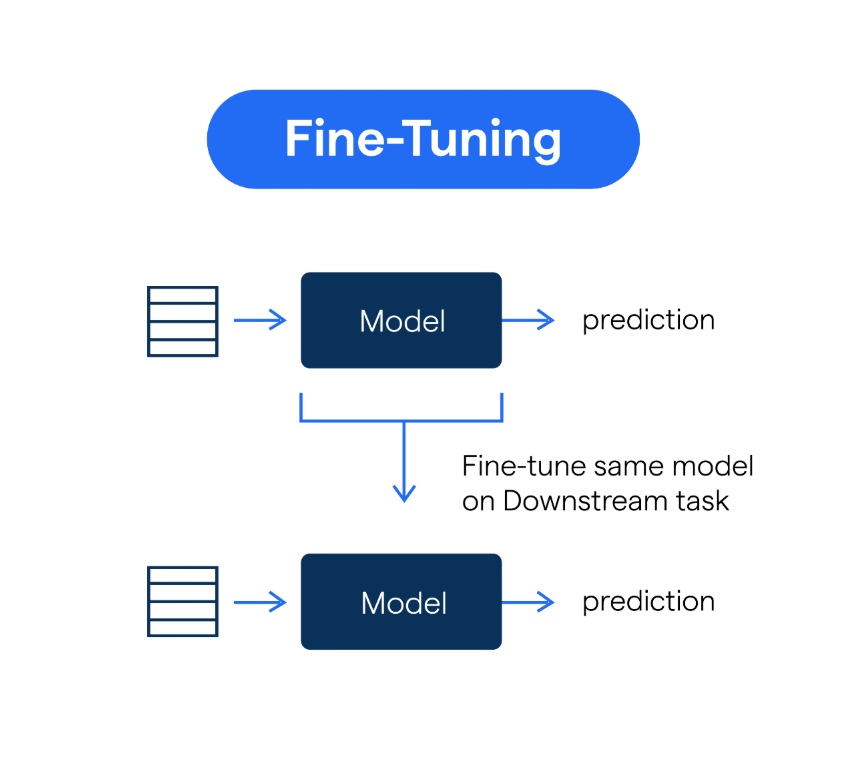
\includegraphics[width=0.8\textwidth]{Figs/fine tuning.png} 
    \caption[Schema del processo di Fine-Tuning]{\small \textbf{Schema del processo di Fine-Tuning.} L'illustrazione mostra la transizione di un modello linguistico da una configurazione generica a una specializzata. Partendo da un modello pre-addestrato che genera predizioni standard, il processo prevede un ulteriore addestramento su un dataset specifico (\textit{downstream task}) per ottimizzare i parametri e adattare il comportamento del sistema a compiti o domini verticali mirati.}
    \label{fig:fine_tuning_schema}
\end{figure}

A differenza del pre-training, il fine-tuning si fonda sull’impiego di dati \textbf{etichettati}: a ogni input è associata un’annotazione esplicita, fornita da un agente esterno — tipicamente un annotatore umano o un sistema automatico di labeling — che rappresenta la risposta corretta o la classe di appartenenza del dato. Tali etichette fungono da segnale di apprendimento diretto, consentendo al modello di aggiornare i propri parametri in modo guidato e di ridurre l’ambiguità interpretativa tipica dei modelli generalisti.

Dal punto di vista metodologico, il fine-tuning può assumere forme differenti a seconda del compito da svolgere. Nei problemi di classificazione, ad esempio, il modello viene ottimizzato per associare correttamente un input a una categoria predefinita; nei compiti di \textit{question answering} o di generazione controllata del testo, l’obiettivo è invece massimizzare la coerenza e la correttezza delle risposte rispetto alle annotazioni fornite. In tutti i casi, la funzione di perdita è progettata per penalizzare le discrepanze tra l’output del modello e le etichette di riferimento, rafforzando progressivamente i comportamenti desiderati.

L’importanza del fine-tuning risiede nella sua capacità di \textbf{specializzare} il modello senza dover ripetere l’intero processo di pre-training. Un LLM generico può così essere adattato a domini verticali quali l’ambito legale, medico, finanziario o ingegneristico, acquisendo familiarità con il linguaggio tecnico, le convenzioni formali e le tipologie di problemi caratteristiche di ciascun settore. Questo approccio consente di ottenere modelli altamente performanti anche in presenza di dataset relativamente piccoli, sfruttando la conoscenza latente già appresa nella fase precedente.

Tuttavia, il fine-tuning tradizionale presenta alcune criticità. Una delle più rilevanti è il fenomeno del \textit{catastrophic forgetting}, ovvero la tendenza del modello a perdere parte delle competenze generali acquisite durante il pre-training quando viene ottimizzato in modo intensivo su un dominio ristretto. Inoltre, l’aggiornamento di tutti i parametri di un LLM comporta un costo computazionale elevato e richiede significative risorse hardware, rendendo il processo poco scalabile in molti contesti applicativi.

Per affrontare tali limitazioni, negli ultimi anni sono state sviluppate tecniche di \textbf{Parameter-Efficient Fine-Tuning} (PEFT), tra cui spicca LoRA (\textit{Low-Rank Adaptation}) \cite{hu2021lora}. Questi approcci mirano a congelare la maggior parte dei parametri del modello di base e ad addestrare solo un sottoinsieme ridotto di pesi aggiuntivi, spesso organizzati in matrici a rango ridotto. Lavori precedenti avevano esplorato direzioni analoghe tramite adapter layers \cite{houlsby2019parameter}, prefix tuning \cite{li2021prefix} e prompt tuning \cite{lester2021power}. In questo modo, è possibile adattare il modello a nuovi compiti riducendo drasticamente il consumo di memoria, il tempo di addestramento e il rischio di perdita delle capacità generali.

Il fine-tuning rappresenta un passaggio fondamentale per trasformare un modello linguistico generico in uno strumento realmente utile in contesti applicativi concreti. Esso funge da ponte tra la conoscenza generale appresa durante il pre-training e le esigenze specifiche del mondo reale, ponendo le basi per ulteriori fasi di ottimizzazione e allineamento orientate all’interazione efficace e affidabile con l’utente finale.


\begin{comment}
\subsection{Instruction Tuning}

L'\textbf{Instruction Tuning} rappresenta una forma evoluta di fine-tuning, fondamentale per rendere i modelli realmente utilizzabili dagli utenti finali sotto forma di assistenti digitali. Senza questa fase, un modello pre-addestrato tenderebbe a "completare" un comando piuttosto che a "eseguirlo" (ad esempio, davanti alla domanda "Qual è la capitale della Francia?", un base model potrebbe rispondere continuando la lista con "Qual è la capitale della Germania?").

Attraverso l'Instruction Tuning, il modello viene esposto a dataset composti da coppie di \textbf{istruzione-risposta}. Questo processo insegna al modello a interpretare l'intento dell'utente e a conformarsi a uno specifico formato di output. Questa tecnica è spesso il prerequisito per fasi successive di allineamento, come il \textit{Reinforcement Learning from Human Feedback} (RLHF). 

\begin{figure}[htbp]
    \centering
    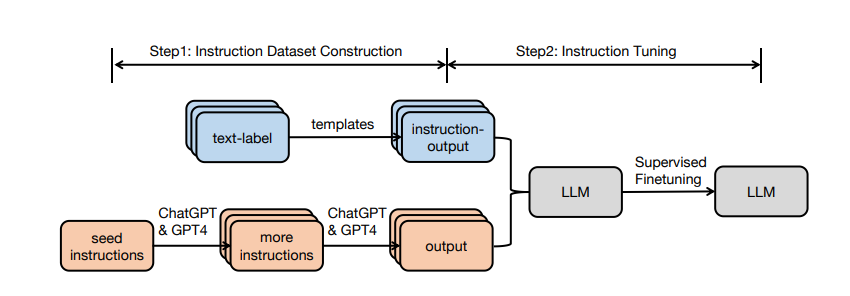
\includegraphics[width=0.8\textwidth]{Figs/pipeline generica di instruction tuning.png}
    \caption{\small Panoramica della pipeline di \textit{Instruction Tuning}.}
    \label{fig:instruction_tuning_pipeline}
\end{figure}

L'\textbf{Instruction Tuning} e la \textbf{Knowledge distillation} sono collegati, siccome molti approcci di Instruction Tuning si basano sulla distillation di modelli di grandi dimensioni, utilizzati come teacher per generare dati di addestramento di alta qualità destinati a modelli più piccoli e più efficienti.

La \textbf{Knowledge Distillation} esercita un'influenza significativa sull'Instruction Tuning, poiché non solo permette di trasferire la conoscenza di un modello ma anche la capacità di ragionamento e di strutturazione delle risposte da un modello \textit{teacher} a uno \textit{student}. In questo contesto, il modello di grandi dimensioni, spesso già allineato tramite Instruction Tuning o RLHF, viene impiegato per generare risposte di alta qualità a un ampio insieme di istruzioni, crando un dataset sintetico che guida l'addestramento di modelli più piccoli ed efficienti.

Molti approcci moderni di \textbf{Instruction Tuning} possono essere interpretati come una forma implicita di distillation, in cui il comportamento desiderato del modello non è appreso direttamente da annotazioni umane, ma viene approssimato replicando le risposte e i pattern decisionali di un modello più performante.

L'influenza della distillation sull'Instruction Tuning risulta particolarmente importante anche sul piano pratico. L'utilizzo di dati generati da modelli \textit{teacher} consente di ridurre significativamente i costi di raccolta di dataset annotati manualmente, migliorando al contempo la qualità e la coerenza delle risposte apprese. Inoltre, tale approccio favorisce la scalabilità del processo di allineamento, rendendo possibile l'addestramento di modelli instruction-tuned destinati a operare su dispositivi o architetture con risorse computazionali limitate.

\end{comment}

\subsection{Instruction Tuning}

L'\textbf{Instruction Tuning} rappresenta una forma evoluta di fine-tuning, fondamentale per rendere i modelli realmente utilizzabili dagli utenti finali sotto forma di assistenti digitali. Senza questa fase, un modello pre-addestrato tenderebbe a ``completare'' un comando piuttosto che a ``eseguirlo'' (ad esempio, davanti alla domanda ``Qual è la capitale della Francia?'', un base model potrebbe rispondere continuando la lista con ``Qual è la capitale della Germania?''). Attraverso l'Instruction Tuning \cite{wei2022finetuned,wang2022self}, il modello viene esposto a dataset composti da coppie di \textbf{istruzione-risposta}: come mostrato in Figura~\ref{fig:instruction_tuning_pipeline}, la pipeline prevede tipicamente la raccolta di istruzioni eterogenee, la generazione delle risposte corrispondenti e il successivo fine-tuning del modello base su questo insieme strutturato. Questo processo insegna al modello a interpretare l'intento dell'utente e a conformarsi a uno specifico formato di output, ed è spesso il prerequisito per fasi successive di allineamento, come il \textit{Reinforcement Learning from Human Feedback} (RLHF) \cite{ouyang2022training}.

L'\textbf{Instruction Tuning} e la \textbf{Knowledge Distillation} sono strettamente collegati: molti approcci moderni si basano sulla distillazione di modelli di grandi dimensioni, utilizzati come \textit{teacher} per generare dati di addestramento di alta qualità destinati a modelli più piccoli ed efficienti. La Knowledge Distillation non permette infatti di trasferire solo la conoscenza fattuale, ma anche la capacità di ragionamento e di strutturazione delle risposte. In questo contesto, il modello \textit{teacher} — spesso già allineato tramite Instruction Tuning o RLHF — viene impiegato per generare risposte ad un ampio insieme di istruzioni, creando un dataset sintetico che guida l'addestramento dello \textit{student}. Molti approcci moderni di Instruction Tuning possono pertanto essere interpretati come una forma implicita di distillazione, in cui il comportamento desiderato non è appreso direttamente da annotazioni umane, ma viene approssimato replicando i pattern decisionali del modello più performante.

Questa sinergia risulta rilevante anche sul piano pratico: l'utilizzo di dati generati dal \textit{teacher} consente di ridurre significativamente i costi di raccolta di dataset annotati manualmente, migliorando al contempo la qualità e la coerenza delle risposte apprese. Inoltre, tale approccio favorisce la scalabilità del processo di allineamento, rendendo possibile l'addestramento di modelli instruction-tuned destinati a operare su dispositivi o architetture con risorse computazionali limitate.

\begin{figure}[t]
    \centering
    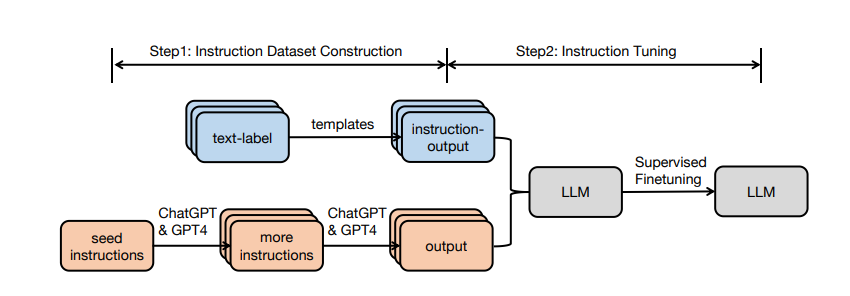
\includegraphics[width=0.8\textwidth]{Figs/pipeline generica di instruction tuning.png}
    \caption{Panoramica della pipeline di \textit{Instruction Tuning}.}
    \label{fig:instruction_tuning_pipeline}
\end{figure}

\section{Knowledge Distillation}

La \textbf{Knowledge Distillation} (KD) rappresenta una delle tecniche più efficaci per la compressione dei modelli, permettendo di trasferire le capacità di un'architettura vasta e complessa (\textbf{Teacher}) a una più compatta ed efficiente (\textbf{Student}). La KD non si basa esclusivamente sull'apprendimento da dati etichettati, ma introduce un cambio di paradigma basato sulla qualità dell'informazione trasmessa.

Il successo di questa tecnica risiede nel superamento del concetto di "etichetta rigida" (\textit{hard target}) tipico del fine-tuning classico. Mentre in un dataset standard ogni esempio è associato a una verità univoca (dove la classe corretta ha probabilità 1 e le altre 0), la distillazione attinge alla cosiddetta \textbf{Dark Knowledge}. Come teorizzato da \citet{hinton2015distilling}, questa "conoscenza oscura" è racchiusa nelle distribuzioni di probabilità prodotte dal modello Teacher, i cosiddetti \textbf{soft targets}. 


\begin{figure}[t]
    \centering
    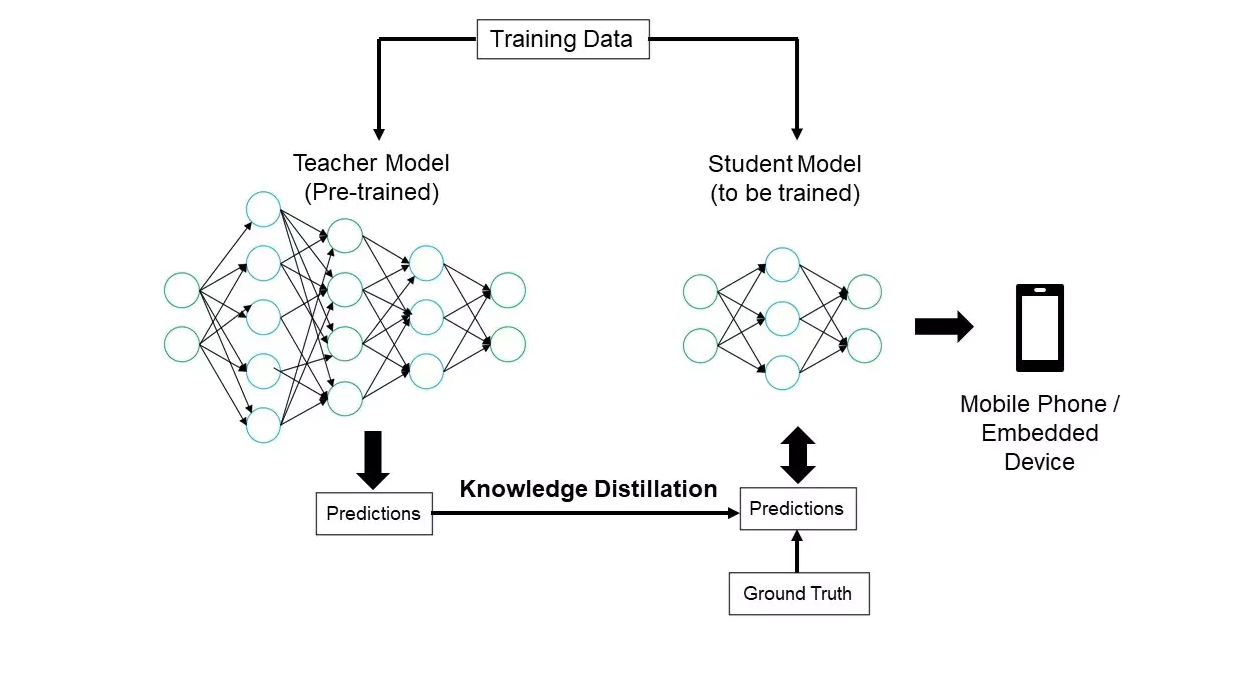
\includegraphics[width=0.8\textwidth]{Figs/distillation.png} 
    \caption[Schema del processo di Knowledge Distillation]{\small \textbf{Rappresentazione del processo di Knowledge Distillation.} Il framework illustra il trasferimento di conoscenza da un \textit{Teacher Model} (pre-addestrato e di grandi dimensioni) a uno \textit{Student Model} più compatto. Attraverso il confronto delle predizioni e l'integrazione con la \textit{Ground Truth}, lo studente viene ottimizzato per operare su dispositivi con risorse limitate, come smartphone o sistemi embedded, mantenendo prestazioni paragonabili al modello più complesso.}
    \label{fig:knowledge_distillation}
\end{figure}


Analizzando i soft targets, lo studente non impara solo qual è la risposta corretta, ma apprende le relazioni semantiche tra le classi. Ad esempio, se il Teacher assegna una probabilità residua più alta alla classe "cane" rispetto alla classe "gatto" mentre analizza l'immagine di un lupo, sta comunicando allo studente una gerarchia di somiglianza che un'etichetta binaria ometterebbe. Per estrarre efficacemente questa conoscenza, viene applicato un parametro di \textbf{Temperatura} ($T$) alla funzione \textit{softmax}:

\begin{equation}
    P_i = \frac{\exp(z_i / T)}{\sum_{j} \exp(z_j / T)}
\end{equation}

L'innalzamento della temperatura ($T > 1$) durante la fase di training permette di "ammorbidire" la distribuzione di probabilità, rendendo più evidenti le sfumature decisionali del Teacher. In questo modo, lo Student può emulare il comportamento logico del modello più grande, raggiungendo prestazioni comparabili pur operando con una frazione dei parametri e delle risorse computazionali. La Knowledge Distillation si configura quindi non solo come uno strumento di efficienza, ma come un processo di raffinamento qualitativo del sapere appreso.

\subsection{Definizione e principi fondamentali}

La \textbf{Knowledge Distillation} (KD) va ben oltre la semplice compressione di un modello riducendone i parametri. È piuttosto un processo elegante e sofisticato che permette di trasferire l’«intelligenza» statistica accumulata da un modello grande (il teacher) a uno più piccolo e leggero (lo student). In pratica, non ci limitiamo a rendere il modello più veloce o meno costoso: cerchiamo di fargli «capire» e ragionare in modo simile a come lo fa il modello più capace, imparando non solo le risposte corrette, ma anche il modo in cui il teacher arriva a quelle risposte. Il principio cardine, formalizzato da \citet{hinton2015distilling}, risiede nell'osservazione che il comportamento di un modello complesso (\textit{Teacher}) contiene informazioni molto più ricche rispetto alle semplici etichette binarie presenti nei dataset tradizionali. Mentre il fine-tuning classico minimizza l'errore rispetto a una \textit{ground truth} rigida (dove una sola classe è corretta e le altre sono considerate parimenti errate), la KD sfrutta la \textbf{Dark Knowledge}.

Questa "conoscenza oscura" è codificata nelle probabilità relative che il \textit{Teacher} assegna alle classi errate. Se, in un compito di classificazione testuale, il \textit{Teacher} assegna una probabilità dello $0.1\%$ alla categoria "sport" e dello $0.0001\%$ alla categoria "cucina" per un testo che parla di "salute", sta comunicando allo \textit{Student} che l'argomento salute è semanticamente più vicino allo sport che alla cucina. Questo segnale di supervisione supplementare permette allo \textit{Student} di apprendere la geometria dello spazio latente del \textit{Teacher}, portando a una generalizzazione superiore.

Dal punto di vista matematico, l'efficacia del trasferimento è regolata dalla funzione di \textbf{Loss di Distillazione}. Lo \textit{Student} viene addestrato minimizzando una funzione di costo composta:
\begin{equation}
    \mathcal{L} = (1 - \alpha) \mathcal{L}_{CE}(y, \sigma(z_s)) + \alpha T^2 \mathcal{L}_{KL}(\sigma(z_t/T), \sigma(z_s/T))
\end{equation}
dove $\mathcal{L}_{CE}$ è la \textit{cross-entropy} standard rispetto alle etichette reali $y$, mentre $\mathcal{L}_{KL}$ è la divergenza di Kullback-Leibler tra le distribuzioni del docente ($z_t$) e dello studente ($z_s$). Il parametro $\alpha$ bilancia l'importanza dei due segnali, mentre la temperatura $T$ gioca un ruolo cruciale: all'aumentare di $T$, la distribuzione dei \textit{logits} si appiattisce, forzando lo \textit{Student} a prestare attenzione non solo al picco di probabilità, ma anche alle relazioni di somiglianza tra le classi meno probabili.

\subsection{Paradigma Teacher--Student}

Il paradigma \textbf{Teacher--Student} non rappresenta soltanto una tecnica di compressione, ma definisce una vera e propria relazione pedagogica tra architetture neurali con obiettivi divergenti. Il \textbf{Teacher} si configura tipicamente come un modello sovra-parametrizzato, come GPT-4 \cite{achiam2023gpt4} o LLaMA \cite{touvron2023llama}, che ha raggiunto la saturazione prestazionale durante il pre-training grazie a centinaia di miliardi di parametri. Sebbene tale complessità garantisca una straordinaria capacità di generalizzazione, essa si traduce in un'inefficienza computazionale critica in termini di latenza e occupazione di memoria VRAM, rendendo il modello difficilmente utilizzabile in scenari \textit{edge} o in tempo reale.

In questo contesto, lo \textbf{Student} emerge come un'architettura snella progettata per operare entro vincoli hardware stringenti, come illustrato in Figura~\ref{fig:teacher_student_architecture}. La sua genesi può seguire percorsi differenti: da un lato la \textit{riduzione strutturale}, in cui lo Student eredita la topologia del Teacher riducendo però il numero di layer, le teste di attenzione o la dimensione degli embedding; dall'altro, l'adozione di \textit{architetture eterogenee}, dove la conoscenza viene trasposta in modelli ottimizzati per specifici processori, come il passaggio da un trasformatore massivo a una rete convoluzionale o a una ricorrente (RNN) più agile.

Un elemento di criticità in questa transizione è rappresentato dal \textbf{Capacity Gap}. Qualora il divario tra le capacità dei due modelli sia eccessivo, lo Student può fallire nell'imitazione poiché le funzioni decisionali del Teacher risultano troppo complesse per essere approssimate da un numero limitato di parametri. Per mitigare questo fenomeno, la letteratura suggerisce l'impiego della \textit{Multi-stage Distillation} o l'introduzione di un \textit{Teacher Assistant} \cite{mirzadeh2020improved}: un modello di taglia intermedia che funge da ponte cognitivo, facilitando un trasferimento graduale della conoscenza e riducendo la perdita di accuratezza finale.

\begin{figure}[t]
    \centering
    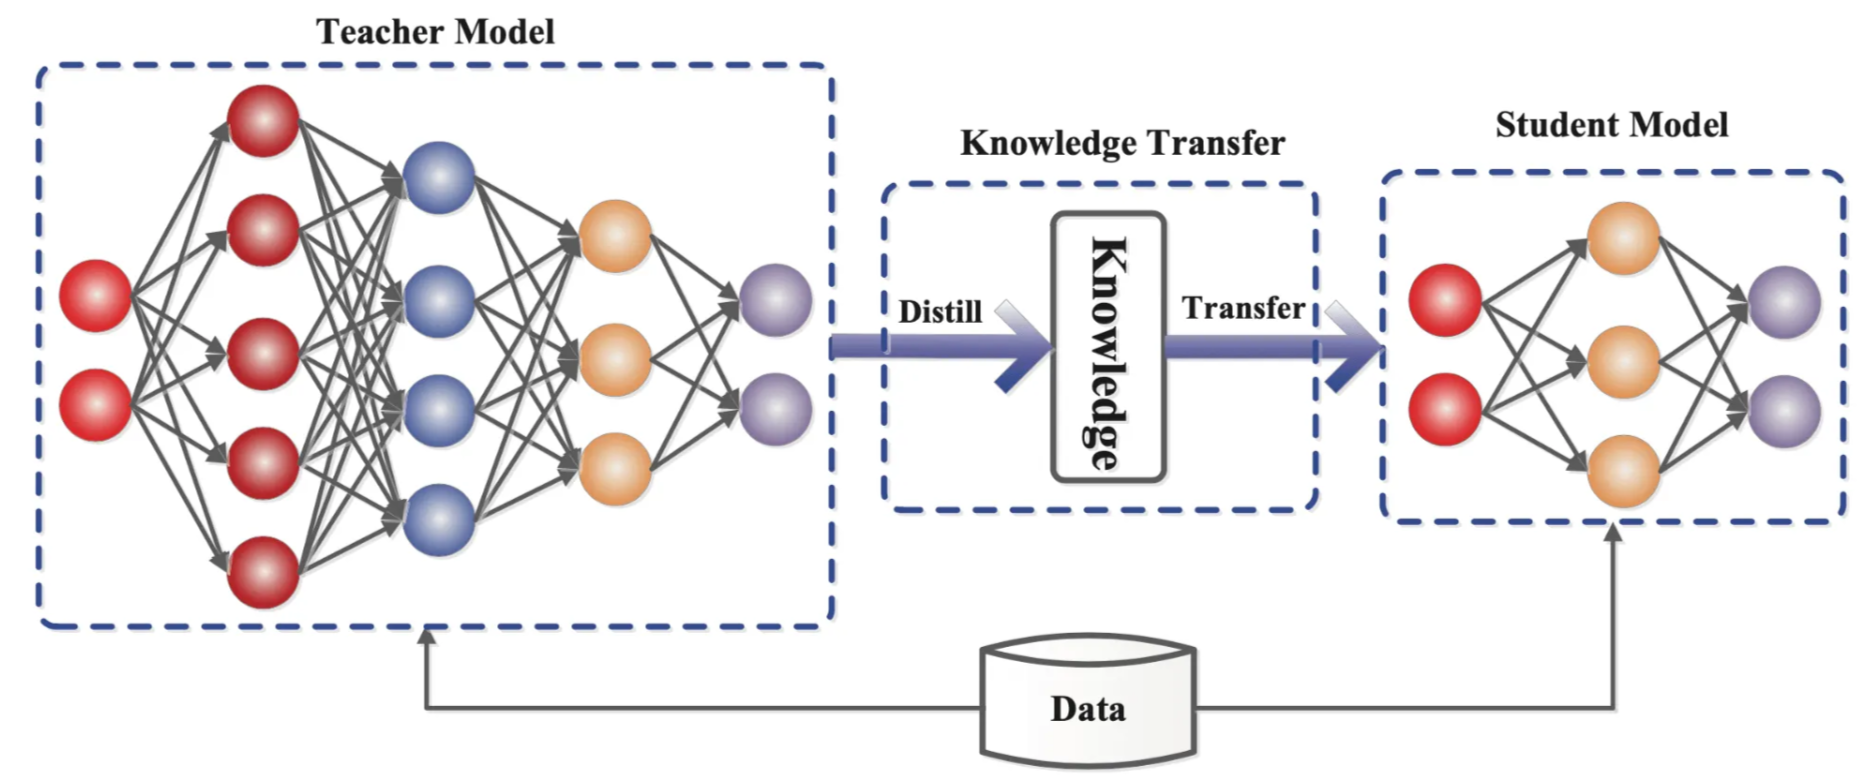
\includegraphics[width=0.8\textwidth]{Figs/teacher-student.png}
    \caption{Architettura di trasferimento della conoscenza da un modello \textit{Teacher} a uno \textit{Student} di dimensioni ridotte.}
    \label{fig:teacher_student_architecture}
\end{figure}

\subsection{Modalità di trasferimento della conoscenza}

Il trasferimento della conoscenza può essere declinato attraverso diverse metodologie operative che variano in base al livello di introspezione richiesto sul modello docente. La forma più accessibile è la \textbf{Response-based Distillation}, comunemente nota come \textit{Logits Distillation}. In questo scenario, lo Student si focalizza esclusivamente sull'output finale, cercando di replicare le distribuzioni di probabilità prodotte dal Teacher. Tale approccio è particolarmente vantaggioso quando si opera con modelli proprietari accessibili solo tramite API, poiché non richiede l'accesso ai pesi interni o alle attivazioni del sistema sorgente. Tuttavia, questa modalità è anche la più superficiale: cattura solo il comportamento esterno del modello senza comprendere i meccanismi interni che hanno portato a quella decisione.

Andando più in profondità, la \textbf{Feature-based Distillation} (o \textit{Hint Training}) \cite{romero2015fitnets} mira ad allineare le rappresentazioni intermedie dei due modelli. Poiché i layer interni catturano astrazioni semantiche e sintattiche fondamentali, lo Student viene forzato a produrre attivazioni simili a quelle del docente in strati specifici della rete. 

\begin{figure}[t]
    \centering
    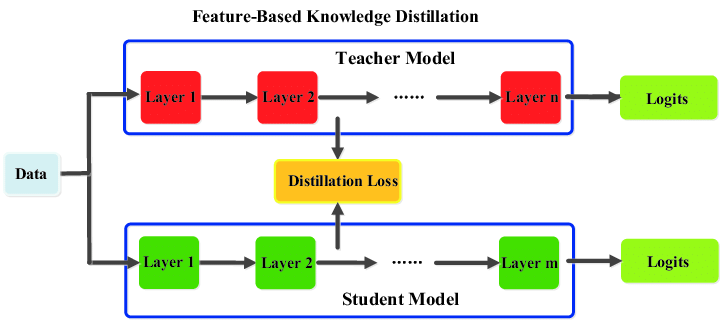
\includegraphics[width=0.8\textwidth]{Figs/The-generic-feature-based-knowledge-distillation.png}
    \caption{\small Architettura concettuale della \textit{Feature-Based Knowledge Distillation}. Il processo prevede il trasferimento di conoscenza attraverso l'allineamento delle mappe di caratteristiche intermedie (feature maps) prodotte dai livelli interni del modello \textit{Teacher} e del modello \textit{Student}. La \textit{Distillation Loss} viene calcolata per minimizzare la discrepanza tra le rappresentazioni latenti dei due modelli durante la fase di addestramento.}
    \label{fig:feature_based_kd}
\end{figure}

Questo approccio permette di trasmettere non solo il \textit{cosa} (l'output finale), ma anche il \textit{come} — ovvero la struttura gerarchica con cui l'informazione viene elaborata. Data la frequente discrepanza dimensionale tra i layer dei due modelli — ad esempio tra un Teacher da 4096 neuroni e uno Student da 768 — si ricorre all'uso di \textit{regressor layer} o proiezioni lineari che mappano lo spazio latente dello Student in quello del Teacher, permettendo un confronto diretto tra le mappe di caratteristiche. Sebbene più efficace della semplice imitazione degli output, questa tecnica richiede accesso completo all'architettura del Teacher e comporta un costo computazionale maggiore durante l'addestramento.

Un'ulteriore evoluzione è rappresentata dalla \textbf{Relation-based Distillation} \cite{park2019relational}, che sposta l'attenzione dai singoli punti dati alle relazioni intercorrenti tra essi. 
Invece di imitare una singola risposta o una singola attivazione, lo Student apprende come il Teacher correla diversi esempi all'interno di un batch o come struttura l'attenzione tra i token in una sequenza. Attraverso l'estrazione di matrici di similarità o mappe di \textit{Self-Attention}, lo Student acquisisce la capacità di pesare l'importanza dei contesti in modo analogo al docente. Questa modalità si rivela particolarmente efficace nei modelli Transformer, dove il meccanismo di attenzione codifica esplicitamente le dipendenze strutturali tra le parole, consentendo allo studente di ereditare pattern di ragionamento relazionale complessi che emergono solo dall'interazione tra più esempi.

\begin{figure}[htbp]
    \centering
    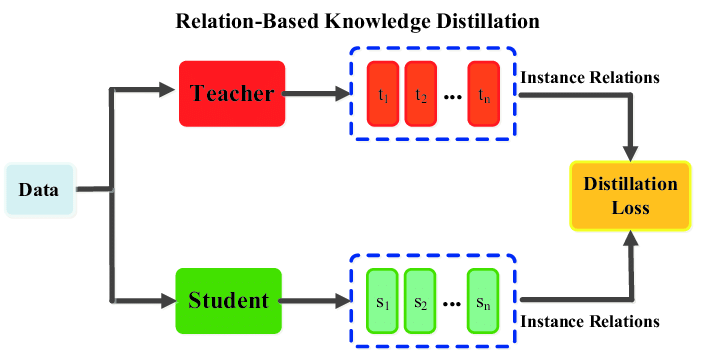
\includegraphics[width=0.8\textwidth]{Figs/The-generic-instance-relation-based-knowledge-distillation.png}
    \caption{\small Schema generale del processo di \textit{Relation-Based Knowledge Distillation}. Il dataset viene processato parallelamente dal modello Teacher e dal modello Student. La distillazione avviene minimizzando la discrepanza tra le relazioni inter-istanza (distanze o similarità tra i campioni $t_n$ e $s_n$) apprese dai due modelli.}
    \label{fig:feature_distillation}
\end{figure}

Infine, con l'avvento dei modelli di ragionamento avanzato come GPT-4 e i sistemi della famiglia o1, si è imposta la \textbf{Logic and Reasoning Distillation} \cite{hsieh2023distilling}. In questa modalità, il trasferimento riguarda le cosiddette \textit{Chain of Thought} (catene di pensiero) \cite{wei2022chain}: lo Student non apprende solo la risposta corretta, ma viene addestrato a replicare i passaggi logici intermedi — le argomentazioni, le verifiche e i ragionamenti controfattuali — che il Teacher esplicita prima di giungere alla conclusione finale. Questo approccio acquisisce capacità di \textit{problem-solving} strutturato che trascendono la mera distribuzione statistica dei token, avvicinando il modello compresso a una forma di ragionamento simbolico implicito.

Va sottolineato che queste strategie non sono mutuamente esclusive. Molti lavori recenti combinano più livelli di distillazione simultaneamente: si può, ad esempio, applicare una perdita sui logits finali insieme a una perdita sulle rappresentazioni intermedie e sulle matrici di attenzione, pesando opportunamente i diversi contributi nella funzione obiettivo complessiva. La scelta della strategia dipende da un trade-off tra accessibilità del Teacher, complessità computazionale dell'addestramento e fedeltà del trasferimento desiderata. L'integrazione sinergica di queste tecniche trasforma la Knowledge Distillation in un pilastro fondamentale per la democratizzazione dell'intelligenza artificiale, permettendo di distribuire capacità di ragionamento sofisticate su dispositivi di consumo quotidiano.

\section{Reflection Tuning}

Il \textbf{Reflection Tuning} \cite{ze2023reflection} rappresenta un'evoluzione paradigmatica nel campo dell'addestramento dei Large Language Models (LLM), spostando il focus dalla mera generazione di testo alla strutturazione del pensiero critico. Mentre l'approccio standard all'Instruction Tuning si limita a ottimizzare il modello affinché produca risposte conformi a un dato input, il Reflection Tuning mira a internalizzare un processo di supervisione cognitiva. Tale metodologia affronta uno dei limiti intrinseci dei modelli basati su Transformer: la natura "unidirezionale" e immediata del campionamento dei token, che spesso porta a errori logici dovuti alla mancanza di una fase di pianificazione o revisione interna.

\subsection{Concetto di self-reflection nei modelli linguistici}

Il concetto di \textbf{self-reflection} nell'ambito dell'intelligenza artificiale non rappresenta una semplice espansione algoritmica, ma un cambio di paradigma che si ispira direttamente alle capacità metacognitive umane. Tale processo definisce la facoltà del modello di monitorare, valutare e regolare i propri processi di pensiero in tempo reale. Nei modelli linguistici tradizionali, l'inferenza avviene solitamente in modo ``greedy'' o stocastico, dove ogni token viene generato in una sequenza lineare senza possibilità di revisione. La riflessione rompe questa linearità introducendo una pausa computazionale strategica: il modello esamina le proprie premesse e valuta la coerenza delle proprie deduzioni prima di cristallizzarle in un output definitivo.

Dal punto di vista della psicologia cognitiva, questo approccio implementa il cosiddetto \textbf{Dual Process Theory} proposto da \citet{kahneman2011thinking}. Mentre i modelli standard operano principalmente in modalità \textit{Sistema 1} — caratterizzata da una risposta veloce, istintiva e basata su pattern statistici immediati — la self-reflection abilita il \textit{Sistema 2}. Quest'ultimo è lento, deliberativo e analitico, e permette al modello di allocare una quota maggiore di risorse computazionali, definita \textit{Inference-time Compute}, per risolvere ambiguità semantiche o complessità logiche che richiederebbero una visione d'insieme superiore a quella offerta dalla semplice previsione del token successivo.

Tecnicamente, la riflessione si realizza attraverso la generazione di una ``traccia di pensiero'' (\textit{reasoning trace}) che funge da memoria di lavoro dinamica. Come illustrato in Figura~\ref{fig:riflection_tuning}, il processo di Reflection Tuning articola l'interazione tra \textit{Teacher} e \textit{Student Model} in tre fasi sequenziali: una prima fase di riflessione selettiva sulle istruzioni, una seconda di riflessione selettiva sulla risposta, e una terza di Instruction Tuning finale sul dataset curato. Durante ciascuna di queste fasi, il modello opera una scomposizione del task, suddividendo istruzioni articolate in sotto-obiettivi atomici affrontati sequenzialmente, filtrando i dati in base a difficoltà e fattibilità. Questo meccanismo permette di verificare la coerenza interna, controllando se i passaggi intermedi contraddicano i dati forniti nel prompt o la conoscenza pregressa memorizzata nei pesi sinaptici. Inoltre, il modello può simulare diverse traiettorie di risposta, valutando virtualmente quale percorso conduca alla probabilità logica più elevata prima di impegnarsi nella scrittura. Tale processo riduce drasticamente le cosiddette \textbf{allucinazioni di ragionamento}, poiché la risposta finale non emerge dal nulla, ma poggia su una catena logica precedentemente validata e corretta dal modello stesso.

\begin{figure}[t]
    \centering
    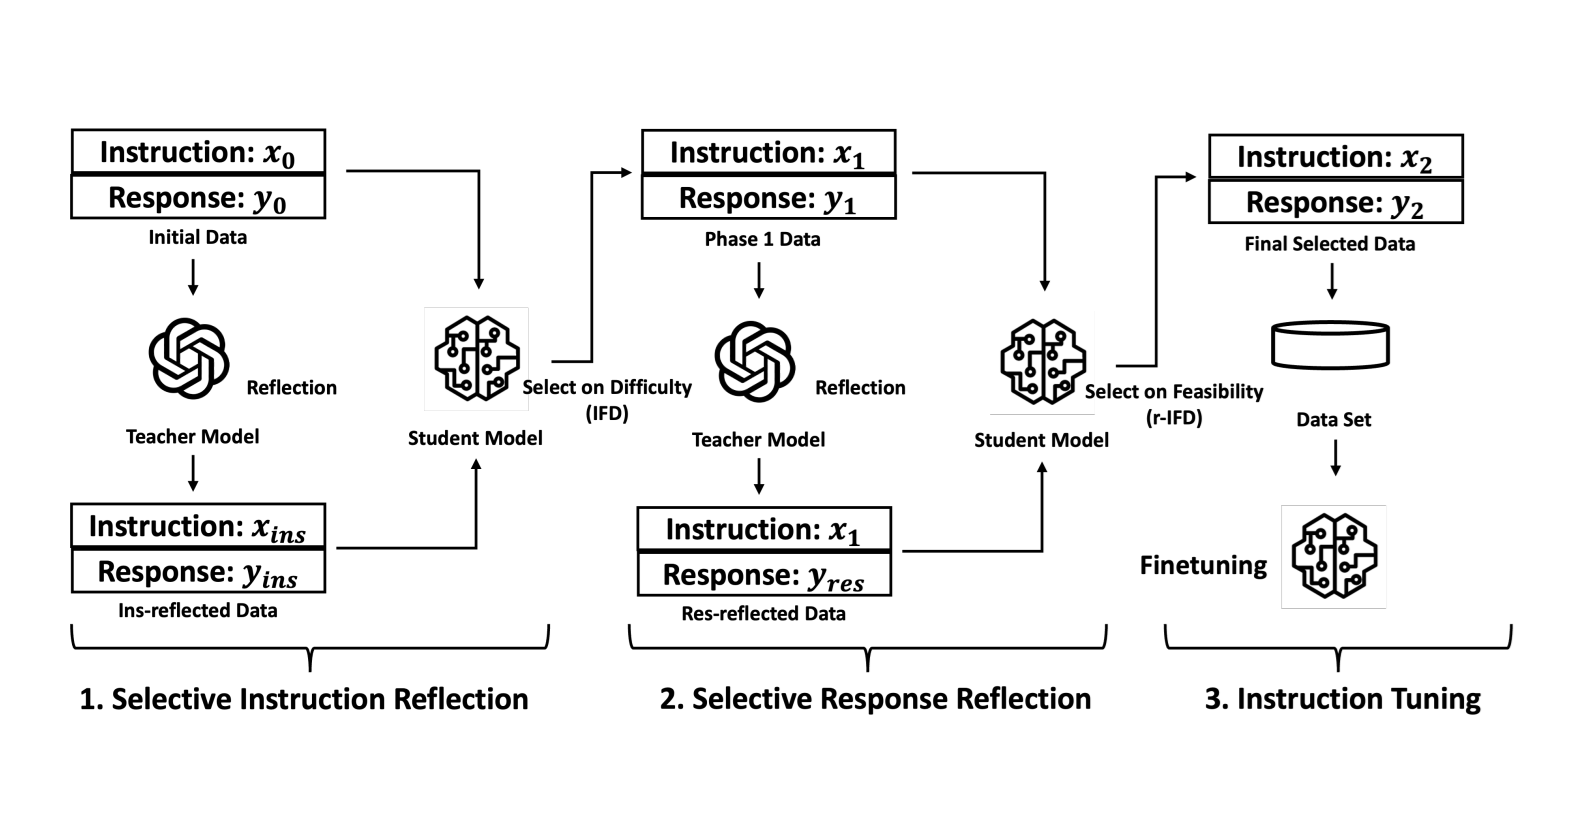
\includegraphics[width=0.8\textwidth]{Figs/Reflection tuning.png}
    \caption{Architettura del processo di \textit{Reflection Tuning}, con l'iterazione tra \textit{Teacher} e \textit{Student Model} nelle tre fasi di riflessione sulle istruzioni, riflessione sulla risposta e \textit{Instruction Tuning} finale sul dataset curato.}
    \label{fig:riflection_tuning}
\end{figure}

\subsection{Reflection Tuning come strategia di training}

Il \textbf{Reflection Tuning} rappresenta l'evoluzione metodologica che trasforma la capacità di riflessione da un comportamento emergente a un obiettivo di addestramento esplicito. A differenza del semplice \textit{Chain-of-Thought prompting} \cite{wei2022chain,kojima2022large}, in cui la riflessione è stimolata solo in fase di inferenza tramite istruzioni testuali (spesso con risultati variabili), il tuning modifica i pesi del modello affinché la riflessione diventi una competenza nativa, strutturale e predicibile. 

L'addestramento si basa su dataset di istruzioni arricchite che seguono una struttura a più stadi, formalizzabile come $\mathcal{D} = \{ (I, R, C, O)_i \}_{i=1}^N$. In questa formulazione, l'istruzione $I$ non porta direttamente all'output $O$, ma transita attraverso una riflessione iniziale $R$ e una fase di correzione $C$. L'inclusione deliberata di errori seguiti da rettifiche all'interno dei dati di addestramento è l'elemento cardine di questa strategia: insegnare al modello a riconoscere un proprio fallimento logico (\textit{error detection}) e a porvi rimedio in autonomia (\textit{error correction}) è ciò che distingue il Reflection Tuning dalle tecniche di fine-tuning convenzionali.



Un aspetto critico risiede nella gestione dei \textbf{token di delimitazione}, che fungono da barriere architettoniche tra il pensiero interno e la risposta esterna. Il modello viene addestrato a utilizzare tag specifici, come \texttt{<thought>}, \texttt{<analysis>} e \texttt{<correction>}, che permettono al sistema di isolare i flussi di elaborazione interna dall'interazione con l'utente, impedendo che i "dubbi" del modello sporchino la qualità del testo finale. 

Durante la fase di ottimizzazione, la funzione di perdita (\textit{loss function}) viene pesata strategicamente per incentivare non solo la correttezza della risposta $O$, ma soprattutto la precisione dei passaggi logici contenuti nella sezione di riflessione. Si assume infatti che la qualità dell'output sia una funzione diretta della qualità del pensiero intermedio. Questo approccio viene spesso potenziato tramite tecniche di \textbf{Reinforcement Learning from Human Feedback} (RLHF) \cite{ouyang2022training} o \textbf{Direct Preference Optimization} (DPO). In questi scenari, i modelli di ricompensa sono istruiti per premiare le tracce di riflessione che dimostrano un rigore metodologico elevato, una verifica accurata dei fatti e la capacità di scartare ipotesi errate, consolidando così un comportamento riflessivo che rende il modello non solo più accurato, ma anche più affidabile e interpretabile.

\subsection{Data recycling e auto-miglioramento}

La frontiera più avanzata del Reflection Tuning risiede nella risoluzione di un paradosso fondamentale: la scarsità di dati di addestramento di alta qualità che includano processi di riflessione espliciti e corretti. Poiché l'annotazione umana di "tracce di pensiero" è un processo estremamente costoso, lento e difficilmente scalabile per compiti di alta complessità scientifica o logica, la ricerca si è orientata verso tecniche di \textbf{Data Recycling} e cicli di \textbf{Auto-miglioramento} (\textit{Self-Improvement}). Queste metodologie permettono ai modelli di generare autonomamente il proprio materiale di studio, innescando un processo di apprendimento ricorsivo che non dipende esclusivamente da input esterni.

Il ciclo di auto-miglioramento si articola tipicamente attraverso un processo iterativo di esplorazione e raffinamento. Inizialmente, di fronte a un insieme di problemi complessi, il modello opera una \textit{generazione di tentativi multipli}, producendo diverse varianti di ragionamento e soluzione. Questo avviene variando la temperatura di campionamento per esplorare percorsi logici eterogenei. Successivamente, queste soluzioni vengono sottoposte a una fase di \textit{verifica tramite oracoli o modelli critici}. In domini deterministici come la matematica o la programmazione, la validazione è oggettiva e automatica, basata sull'accuratezza del risultato finale o sull'esecuzione di test unitari. In ambiti meno strutturati, interviene un modello "critico" (spesso un \textit{Teacher} di dimensioni superiori) con il compito di analizzare la coerenza formale della riflessione.



Il cuore pulsante di questa strategia è il \textit{re-training su dati filtrati}. Solo le traiettorie di pensiero che hanno condotto con successo alla soluzione corretta vengono integrate nel dataset di fine-tuning per il ciclo successivo. Questo meccanismo è alla base di algoritmi seminali come \textbf{STaR} (\textit{Self-Taught Reasoner}) \cite{zelikman2022star}, in cui il modello impara a razionalizzare a posteriori le risposte corrette che inizialmente aveva individuato in modo fortuito. In questo modo, le intuizioni statistiche si cristallizzano in regole logiche consolidate, permettendo al modello di "imparare a pensare" dai propri successi.

Tuttavia, l'autosufficienza del data recycling introduce sfide non trascurabili, in particolare il rischio di \textbf{bias amplification} e la cosiddetta "deriva semantica". Se il modello viene addestrato su riflessioni che contengono errori logici sottili o passaggi ridondanti non rilevati dai filtri, rischia di stabilizzare abitudini di ragionamento fallaci, seppur formalmente eleganti. Per mitigare tale deriva, le architetture più recenti adottano una \textbf{Knowledge Distillation incrociata} \cite{madaan2023self,shinn2023reflexion}. In questo scenario, la capacità di riflessione di modelli ultra-large (come i modelli della serie "o1" o DeepSeek-R1 \cite{deepseekr1_2025}) viene utilizzata per supervisionare e "pulire" i dati sintetici generati dai modelli più piccoli. 

Questo connubio tra auto-generazione e supervisione esterna garantisce che l'auto-miglioramento rimanga ancorato a standard di rigore logico elevati. Il Reflection Tuning cessa così di essere una semplice fase di addestramento statico per trasformarsi in un meccanismo di evoluzione cognitiva autonoma, dove lo Student non si limita a imitare il Teacher, ma utilizza gli strumenti logici acquisiti per esplorare e mappare autonomamente nuovi domini di conoscenza.

\section{LLM-as-a-Judge}
\label{sec:llm_judge}

La valutazione automatica delle risposte generate da modelli linguistici
rappresenta uno dei problemi aperti più rilevanti nell'ambito della
ricerca sugli LLM. Le metriche classiche basate sul confronto lessicale
--- come BLEU, ROUGE o METEOR --- si rivelano inadeguate per testi a
risposta aperta, in cui risposte semanticamente equivalenti possono
differire radicalmente nella formulazione superficiale. L'annotazione
umana, pur restando lo standard di riferimento, è costosa, lenta e
soggetta a variabilità inter-annotatore. Il paradigma
\textbf{LLM-as-a-Judge} \cite{zheng2023judging} propone una soluzione
intermedia: utilizzare un Large Language Model di elevata capacità come
giudice automatico che valuta la qualità delle risposte prodotte da
altri modelli.

L'idea fondamentale è che un LLM sufficientemente capace sia in grado
di apprezzare sfumature qualitative --- correttezza fattuale,
coerenza logica, chiarezza espositiva, utilità della risposta ---
in modo analogo a un valutatore umano esperto, ma a una frazione
del costo e del tempo. Il giudice riceve in input il testo della
domanda, la risposta (o le risposte) da valutare e un insieme di
criteri di giudizio specificati nel prompt di sistema. Produce in
output uno o più punteggi numerici su scale definite e,
facoltativamente, una motivazione testuale della valutazione.

La letteratura distingue tre configurazioni principali. Nel
\textbf{giudizio assoluto} (\textit{pointwise}), il giudice valuta
una singola risposta assegnando un punteggio su una scala discreta
(tipicamente 1--5 o 1--10) per ciascuna metrica di interesse; questa
modalità è adatta a valutare la qualità intrinseca di un modello
senza confronto diretto con altri. Nel \textbf{giudizio comparativo}
(\textit{pairwise}), vengono presentate al giudice le risposte di
due modelli diversi alla stessa domanda; il giudice deve determinare
quale sia preferibile, oppure dichiarare una parità. Questa modalità
riduce i bias di calibrazione assoluta e facilita il ranking relativo
tra sistemi. Infine, nel \textbf{giudizio su lista} (\textit{listwise}),
più risposte vengono ordinate simultaneamente, con il vantaggio di una
maggiore coerenza transitiva ma a costo di un prompt più complesso.

Il principale vantaggio dell'approccio LLM-as-a-Judge è la scalabilità:
permette di valutare migliaia di risposte in tempi ridotti e a costi
contenuti, rendendo possibili esperimenti di valutazione che sarebbero
proibitivi con annotatori umani. Studi empirici hanno mostrato
correlazioni elevate tra i giudizi prodotti da modelli come GPT-4
e le valutazioni umane su diversi benchmark \cite{zheng2023judging}.

Tuttavia, il paradigma presenta criticità note. Il \textbf{position
bias} è la tendenza del giudice a preferire sistematicamente la
risposta presentata per prima (o per ultima) indipendentemente dal
contenuto, mitigabile invertendo l'ordine delle risposte e
aggregando i giudizi. Il \textbf{verbosity bias} è la preferenza
per risposte più lunghe e articolate anche quando una risposta
concisa sarebbe più appropriata. Il \textbf{self-enhancement bias}
descrive la tendenza di un modello a favorire risposte stilisticamente
simili alle proprie, il che introduce un potenziale conflitto di
interessi quando il giudice coincide con il modello teacher usato
per generare i dati di training. Infine, i giudizi possono essere
sensibili alla formulazione del prompt: criteri espressi in modo
ambiguo portano a valutazioni inconsistenti anche a parità di risposta.
Nonostante questi limiti, l'LLM-as-a-Judge è oggi ampiamente adottato
come strumento di valutazione pratico nell'ambito della ricerca
sui modelli linguistici \cite{zheng2023judging}.